%!TEX root = ./icml2016.tex

\section{Compositional Relations}

\begin{figure}[t]
	\centering
	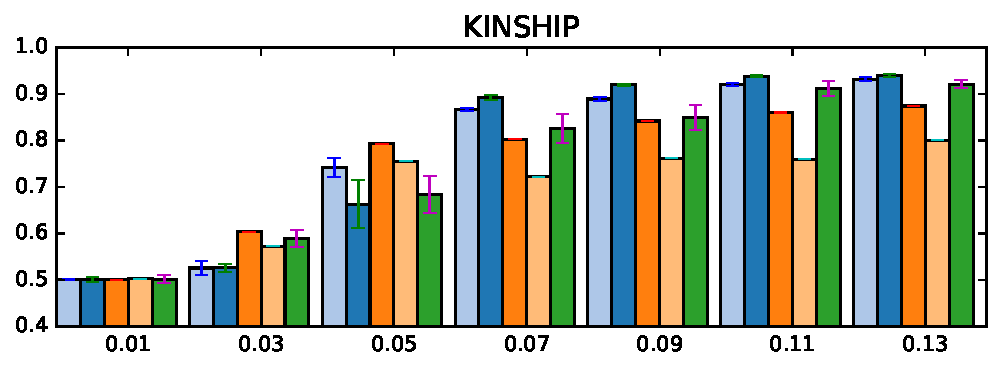
\includegraphics[width=\linewidth]{images/comp_training_error_kinship_small.pdf}
	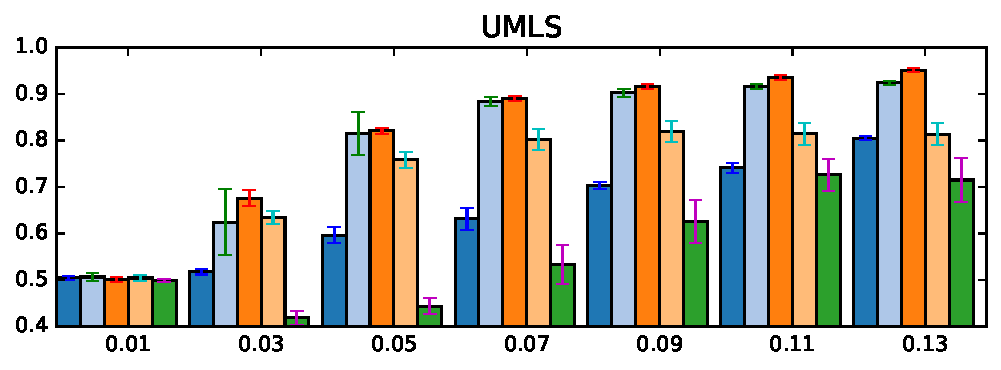
\includegraphics[width=\linewidth]{images/comp_training_error_umls_small.pdf}			
	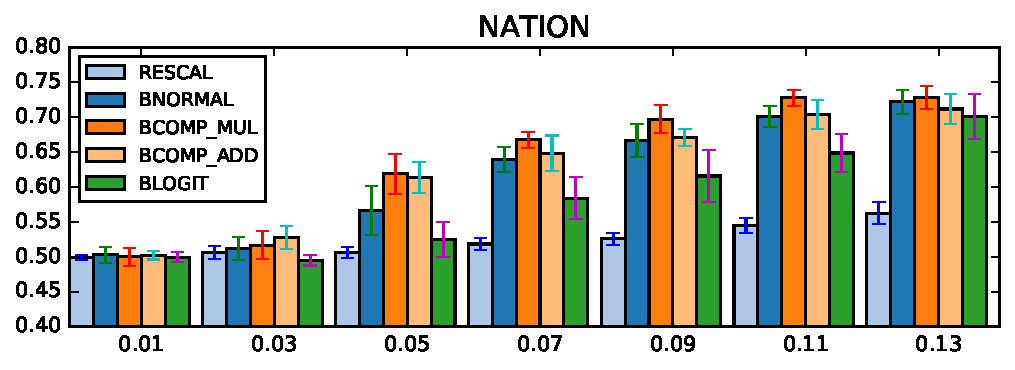
\includegraphics[width=\linewidth]{images/comp_training_error_nation_small.pdf}				
	\caption{\label{fig:r_vs_br} ROC-AUC scores of compositional models. The x-axis denotes the proportion of an observed triples including negative triples used for training models. We  use another 30\% of triples to evaluate the ROC-AUC score. In general, compositional models outperform BRESCAL and BLOGIT model when the size of training set is relatively small, whereas BRESCAL and BLOGIT perform slightly better than or comparable to the compositional models when the size of training set is relatively large. For UMLS dataset, the multiplicative compositional model consistently outperforms the other models across all training proportions.}
\end{figure} 


From two triples:
$(i, k_1 ,j)$,  $(j, k_2, l)$

Compositional triple:
$(i, {c}(k_1, k_2), l)$

This compositional triple may have multiple path over the knowledge graph. For example, both pairs of triples $(i, k_1 ,j)$,  $(j, k_2, l)$ and $(i, k_1 ,m)$,  $(m, k_2, l)$ can be represented as $(i, {c}(k_1, k_2), l)$. To include the compositionality of the knowledge graph, we set  $x_{(i, {{c}(k_1, k_2)}, l)}$ be the number of path from entity $i$ to entity $j$ through relation $k_1$ and $k_2$.

We model a degree of the compositional relation as
\begin{align}
x_{(i, {{c}(k_1, k_2)}, l)} \sim \mathcal{N}(e_i^\top R_{{c}(k_1,k_2)} e_j, \sigma_{c}^2),
\end{align}
where $R_{{c}(k_1,k_2)} \in \mathbb{R}^{D\times D}$.

Let $\mathcal{C}^{L}$ be a set of all possible compositions of which length is up to length $L$, $c \in \mathcal{C}$ be a sequence of compositions, and $c(i)$ be $i$th index of a relation in sequence $c$. With the set of compositions $\mathcal{C}^{L}$, we can expand set of observed triples $\mathcal{X}^{t}$ to set of observed compositional triple $\mathcal{X}^{\mathcal{C}^{L}(t)}$ of which element $x_{icj}$ is a number of path from entity $i$ to entity $j$ through sequence of relations $c$ in $\mathcal{X}^{t}$.

\subsection{Additive Compositionality}
Let $R_{{c}} = \frac{1}{|c|}(R_{c(1)} + R_{c(2)} + \dots + R_{c(|c|)})$, then
\begin{align}
x_{(i, k_{{c}}, l)} \sim \mathcal{N}(e_i^\top R_c e_j, \sigma_{c}^2).
\end{align}

The conditional distribution of $e_i$ given $E_{-i}, \mathcal{R}, \mathcal{X}^{t}, \mathcal{X}^{L(t)}$ is 
\begin{align} \label{eqn:sample_e}
p(e_i |E_{-i}, \mathcal{R}, \mathcal{X}^{t}, \mathcal{X}^{L(t)}) &= \mathcal{N}(e_i | \mu_i, \Lambda_i^{-1}),
\end{align}
where
\begin{align*}
\mu_i &= \Lambda_i^{-1}\xi_i \\
\Lambda_i &= \frac{1}{\sigma_x^2} \sum_{jk : x_{ikj} \in \mathcal{X}^{t}} (R_k e_j)(R_k e_j)^\top \\
&\quad+ \frac{1}{\sigma_x^2} \sum_{jk : x_{jki} \in \mathcal{X}^{t}} (R_k^\top e_j)(R_k^\top e_j)^\top \\
&\quad + \frac{1}{\sigma_c^2} \sum_{jc : x_{icj} \in \mathcal{X}^{L(t)}} (R_c e_j)(R_c e_j)^\top \\
&\quad+ \frac{1}{\sigma_c^2} \sum_{jc : x_{jci} \in \mathcal{X}^{L(t)}} (R_c^\top e_j)(R_c^\top e_j)^\top + \frac{1}{\sigma_e^2} {I}_D \\
\xi_i &= \frac{1}{\sigma_x^2}\sum_{jk : x_{ikj} \in \mathcal{X}^{t}}  x_{ikj} R_{k} e_{j} + \frac{1}{\sigma_x^2}\sum_{jk : x_{jki} \in \mathcal{X}^{t}} x_{jki} R_{k}^\top e_{j} \\
& + \frac{1}{\sigma_c^2}\sum_{jc : x_{icj} \in \mathcal{X}^{L(t)}}  x_{icj} R_{c} e_{j} + \frac{1}{\sigma_c^2}\sum_{jc : x_{jci} \in \mathcal{X}^{L(t)}} x_{jci} R_{c}^\top e_{j}
\end{align*}

To compute the conditional distribution of $R_k$, we first decompose $R_c$ into two part where $R_c = \frac{1}{|c|} R_k + \frac{|c|-1}{|c|}R_{c/k}$, where $R_{c/k} = \sum_{k' \in c/k} R_{k'}$, if compositional sequence $c$ contains relation $k$. Vectorisation of $R_c$ and $R_{c/k}$ are represented as $r_c$ and $r_{c/k}$, respectively.

The degree of compositional path is represented with a decomposition as follows:
\begin{align}
x_{(i, c, l)} \sim \mathcal{N}(e_i^\top (\frac{1}{|c|} R_k + \frac{|c|-1}{|c|}R_{c/k}) e_j, \sigma_{c}^2).
\end{align}

Then, the conditional distribution $R_k$ given $R_{-k}, E, \mathcal{X}^{t}, \mathcal{X}^{L(t)}$ is
\begin{align}
\label{eqn:comp_cond_r}
p(R_k|E, \mathcal{X}^{t}, \mathcal{X}^{L(t)}, \sigma_r, \sigma_x)  &= \mathcal{N}(\text{vec}(R_k) | \mu_k, \Lambda_k^{-1}),
\end{align}
where
\begin{align*}
\mu_k &=\Lambda_k^{-1}\xi_k \\
\Lambda_k &= \frac{1}{\sigma_x^2} \sum_{ij:x_{ikj} \in \mathcal{X}^{t}} \bar{e}_{ij}\bar{e}_{ij}^\top + \frac{1}{\sigma_r^2} {I}_{D^2} \\
& +\frac{1}{|c|^2 \sigma_c^2} \sum_{ij:x_{icj} \in \mathcal{X}^{L(t)},\text{ }k \in c} \bar{e}_{ij} \bar{e}_{ij}^\top \\
\xi_k &=  \frac{1}{\sigma_x^2}\sum_{ij:x_{ikj} \in \mathcal{X}^{t}} x_{ikj} \bar{e}_{ij}\\
& +\frac{1}{|c| \sigma_c^2} \sum_{ij:x_{icj} \in \mathcal{X}^{L(t)},\text{ }k \in c} x_{icj} \bar{e}_{ij} - \frac{|c|-1}{|c|} \bar{e}_{ij} r_{c/k}^\top \bar{e}_{ij}\\
\bar{e}_{ij} &= e_{i} \otimes e_{j}.
\end{align*}

Note that the ordering of the relations in compositional sequence $c$ does not affect the value of compositional triple $(i, c, j)$.

\subsection{Multiplicative Compositionality}
Let compositional relation $R_c = R_{c(1)} R_{c(2)} \dots R_{c(|c|)}$.

If the determinant of latent relation $R_k$ is greater than 1, the compositional latent relation $R_c$ might be exploded after multiplying a long sequence of relations. To obtain a stable scale of compositional relation $R_c$, one may multiply decaying factor $\tau < 1$ after each composition. $R_c = \tau^{|c|-1} R_{c(1)} R_{c(2)} \dots R_{c(|c|)}$.

\begin{align}
x_{(i, c, j)} \sim \mathcal{N}(e_i^\top R_{c(1)}R_{c(2)} \dots R_{c(|c|-1)}R_{c(|c|)} e_j, \sigma_{c}^2)
\end{align}

If the compositional sequence $c$ contains relation $k$, the mean parameter of normal distribution contains $R_k$ in the middle of compositional sequence (i.e., $e_i^\top R_{c(1)}R_{c(2)} \dots R_{c(\delta_k)} \dots R_{c(|c|-1)}R_{c(|c|)} e_j$ where $\delta_k$ is the index of relation $k$). For notational simplicity, we will denote the left side $e_i^\top R_{c(1)}R_{c(2)} \dots R_{c(\delta_k -1)}$ as $\bar{e}_{ic(:\delta_k)}^\top$, and the right side $R_{c(\delta_k + 1)} \dots R_{c(|c|-1)}R_{c(|c|)} e_j$ as $\bar{e}_{ic(\delta_k:)}$, therefore we can rewrite the mean parameter as $\bar{e}_{ic(:\delta_k)}^\top R_{k} \bar{e}_{ic(\delta_k:)}$.

The conditional distribution of $e_i$ given the rest is the same as Equation $\ref{eqn:sample_e}$. The conditional of $R_k$ is
\begin{align}
p(R_k|E, \mathcal{X}, \sigma_r, \sigma_x)  &= \mathcal{N}(\text{vec}(R_k) | \mu_k, \Lambda_k^{-1}),
\end{align}
where
\begin{align*}
\mu_k &= \Lambda_k^{-1}\xi_k \\
\Lambda_k &= \frac{1}{\sigma_x^2} \sum_{ij:x_{ikj} \in \mathcal{X}^{t}} (e_i \otimes e_j)(e_i \otimes e_j)^\top + \frac{1}{\sigma_r^2} {I}_{D^2} \\
+ &\frac{1}{\sigma_c^2} \sum_{ij:x_{icj} \in \mathcal{X}^{L(t)}, \text{ }k \in c} (\bar{e}_{ic(:\delta_k)} \otimes \bar{e}_{jc(\delta_k:)})(\bar{e}_{ic(:\delta_k)} \otimes \bar{e}_{jc(\delta_k:)} )^\top \\
\xi_k &= \frac{1}{\sigma_x^2} \sum_{ij:x_{ikj} \in \mathcal{X}^{t}} x_{ikj} (e_{j} \otimes e_{i}) \\
& + \frac{1}{\sigma_c^2} \sum_{ij:x_{icj} \in \mathcal{X}^{L(t)}, \text{ }k\in c} x_{icj} (\bar{e}_{ic(:\delta_k)}  \otimes \bar{e}_{jc(\delta_k:)}).
\end{align*}


Thoughts: As the length of sequence $c$ increases, a small error in the first few multiplication will result a large differences in the final compositional relation. One way to mitigate this cascading error is to increase the variance of compositional triples as length of sequences increase.

